\documentclass[journal]{IEEEtran}
\usepackage[margin=0.67in]{geometry}
\usepackage{dblfloatfix}
\usepackage{cite}
\usepackage{amssymb}
\usepackage{amsfonts}
\usepackage{amsmath}
\usepackage[T1]{fontenc}
%\usepackage{algorithm}
\usepackage{algpseudocode}
\usepackage[utf8]{inputenc}
\usepackage[english]{babel}
\usepackage[usenames, dvipsnames]{color}
\usepackage{pifont}
\usepackage{booktabs}
%\usepackage{enumitem}
\usepackage{amsmath}
\usepackage{mathtools}
%\usepackage{mathtools}
\usepackage{ellipsis}
\usepackage{textcomp}
\usepackage{cite}
\usepackage[pdftex]{graphicx}
\usepackage{subfigure}
%\usepackage{scalerel}
%\usepackage{subcaption}
\usepackage{epsfig}
\usepackage{epstopdf}
\usepackage{caption}
%\usepackage{algorithm}%\usepackage{algpseudocode}
%\usepackage{algorithmicx}
\usepackage[ruled,vlined,commentsnumbered]{algorithm2e}
\usepackage{fixltx2e}
\usepackage{algpseudocode}
\usepackage{epstopdf}
\usepackage{psfrag}
\usepackage{grffile}
\usepackage{amsthm}
\SetKwInput{KwIn}{Inputs}
\DeclareMathOperator*{\argmax}{arg\,max}
\usepackage[font={footnotesize}]{caption}
\DeclarePairedDelimiter{\ceil}{\lceil}{\rceil}
\newtheorem{thm}{\textbf{Theorem}}
\newtheorem{proposition}{\textbf{Proposition}}
\newtheorem{crl}{Corollary}[section]
\theoremstyle{definition}
\newtheorem{dfn}{Definition}
\theoremstyle{remark}
\newtheorem{note}{Note}[section]
\theoremstyle{plain}
\newtheorem{lem}[thm]{Lemma}
\newcommand{\RNum}[1]{\uppercase\expandafter{\romannumeral #1\relax}}
\usepackage{setspace}
\newcounter{MYtempeqncnt}


\begin{document}
\bstctlcite{IEEEexample:BSTcontrol}
\title{Enabling Intelligent Multi-AP Coordination for Wi-Fi 8}

\author{Deep~Sudhanvabhai~Gajjar,~and~Pradyumna~Kumar~Bishoyi,~\IEEEmembership{Member,~IEEE,}
	\thanks{D. S. Gajjar is with the Department of Electrical Engineering, Indian Institute of Technology Jodhpur, Rajasthan, India, 342030 (email: b23ee1014@iitj.ac.in).}
	\thanks{P. K. Bishoyi is with the Department of Electronics Engineering, Indian Institute of Technology Jodhpur, Rajasthan, India, 342030, (email: pradyumna@iitj.ac.in).}
}

\maketitle

\begin{abstract}
Coordinated spatial reuse (C-SR) is one of the multi-access point coordination (MAPC) modes of IEEE 802.11bn (Wi-Fi 8). In C-SR, the access point (AP) that wins a transmission opportunity (TXOP) shares it with a second AP, and a controller has to select the AP and the station that join the TXOP. We model this selection with a two-level hierarchical multi-armed bandit (H-MAB) and evaluate $\epsilon$-greedy and upper confidence bound (UCB) agents. We then add a weighted per-station urgency term to the selection index, which gives urgency-aware (UA) versions of both agents. In a four-AP deployment, UCB reaches 98.8\% of the oracle data rate, compared with 96.8\% for $\epsilon$-greedy, and obtains half of its final gain in 0.44~s instead of 2.92~s. With urgency, UA-UCB attains 97.7\% of the oracle utility and serves more urgent stations than UA-$\epsilon$-greedy at the same data rate.
\end{abstract}

\begin{IEEEkeywords}
IEEE 802.11bn, Wi-Fi 8, multi-AP coordination, coordinated spatial reuse, multi-armed bandits.
\end{IEEEkeywords}

\IEEEpeerreviewmaketitle
\section{Introduction}
\IEEEPARstart{I}{n} recent years, dense Wi-Fi deployments have made co-channel interference between overlapping basic service sets a major limit on throughput and latency. IEEE 802.11bn (Wi-Fi 8) therefore introduces multi-AP coordination (MAPC) \cite{galati2024wifi8,yu2024spec}. In coordinated spatial reuse (C-SR), the AP that wins a TXOP, called the sharing AP, invites a shared AP to transmit at the same time on the same channel \cite{nunez2022txop,wojnar2025hmab}.

\subsection{Motivation}
The gain of C-SR depends on which AP-station pair is added to the TXOP. Selection based on received signal strength (RSS) reports suffers from RSS variance and signaling overhead \cite{kim2013rss,seok2020csr}. Multi-armed bandits (MABs) avoid this exchange by learning from the outcome of past transmissions \cite{wojnar2025hmab,wojnar2025jsac}. Existing MAB schemes maximize the data rate only, whereas Wi-Fi 8 also targets low latency \cite{galati2024wifi8}, so station urgency should be part of the selection.

\subsection{Literature Survey}
C-SR group selection has been studied with link rate estimation and group scheduling \cite{nunez2022txop,nunez2023group}, RSSI-based SINR prediction \cite{imputato2024beyond}, testbed controllers \cite{haxhibeqiri2024wfcs,haxhibeqiri2024commag}, analytical throughput models \cite{wilhelmi2023throughput} and power control \cite{wang2024fl,talukder2023enhanced}. A survey of MAPC is given in \cite{verma2024survey}. MABs were earlier applied to uncoordinated spatial reuse \cite{bardou2021improving,wilhelmi2019potential,wilhelmi2019collaborative,kim2024contextual,iturria2024cooperate}. Wojnar \textit{et al.} proposed the H-MAB for C-SR and found UCB to perform best \cite{wojnar2025hmab}, and later added transmit power selection and testbed validation \cite{wojnar2025jsac}. In these works the reward is the aggregate data rate.

\subsection{Contributions}
\begin{enumerate}
\item A formulation of two-AP C-SR selection with the sharing pair as context, with oracle bounds for the data rate and for a rate-urgency utility.
\item A comparison of $\epsilon$-greedy and UCB agents in the H-MAB, including the steady-state accuracy limit of $\epsilon$-greedy.
\item Urgency-aware $\epsilon$-greedy and UCB agents that add a weighted urgency term to the selection index and learn only from the data rate.
\end{enumerate}

\section{System Model}\label{sec2}
\subsection{Network and Channel Access}
We consider the downlink of $N$ APs, $\mathcal{A}=\{A_1,\dots,A_N\}$, connected to a central controller \cite{wojnar2025hmab}. AP $A_i$ serves $\mathcal{S}_i=\{S_i^1,\dots,S_i^{m_i}\}$, and $M=\sum_{i=1}^{N}m_i$. Node $X$ is at $\mathbf{p}_X\in\mathbb{R}^2$, and $\delta_{XY}=\|\mathbf{p}_X-\mathbf{p}_Y\|_2$. All stations are backlogged.

Time is divided into TXOPs of duration $\tau$, indexed by $t$. In TXOP $t$, the sharing AP $A_k(t)$ is drawn uniformly from $\mathcal{A}$ and its station $S_k^l(t)$ uniformly from $\mathcal{S}_k$, which models DCF contention \cite{wojnar2025hmab}. The sharing pair is $P_0(t)=(A_k(t),S_k^l(t))$. The controller selects a shared pair $P_1(t)=(A_i(t),S_i^j(t))$ from
\begin{equation}\label{eq:actions}
\mathcal{X}(A_k)=\left\{(A_i,S_i^j): A_i\in\mathcal{A}\setminus\{A_k\},\ S_i^j\in\mathcal{S}_i\right\},
\end{equation}
with $|\mathcal{X}(A_k)|=M-m_k$, and both pairs transmit concurrently.

\begin{figure}[t]
\centering
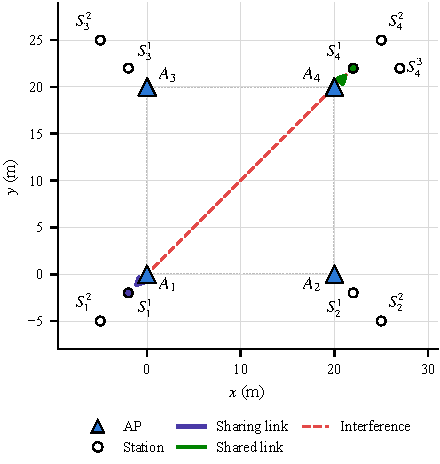
\includegraphics[width=0.8\columnwidth]{fig_topology.pdf}
\caption{Simulated deployment. The arrows show one C-SR configuration with $P_0=(A_1,S_1^1)$ and $P_1=(A_4,S_4^1)$.}
\label{fig:topology}
\end{figure}

\subsection{Propagation and Link Model}
The path loss follows the TGax enterprise model \cite{wojnar2025hmab,merlin2015tgax}:
\begin{equation}\label{eq:pathloss}
\mathrm{PL}(\delta)=L_0+20\log_{10}\bar{\delta}+\mathbf{1}\{\delta>B_p\}\,35\log_{10}\frac{\delta}{B_p}+7W,
\end{equation}
where $\bar{\delta}=\min\{\max\{\delta,1\},B_p\}$, $B_p$ is the breakpoint distance, $W$ is the number of walls and $L_0=40.05+20\log_{10}(f_c/2.4)$ for the carrier frequency $f_c$ in GHz. The received power is $P_{XY}=P_{\mathrm{tx}}-\mathrm{PL}(\delta_{XY})$. For the shared pair $(A_i,S)$, the SINR at $S$ is
\begin{equation}\label{eq:sinr}
\gamma_t=P_{A_iS}-10\log_{10}\left(10^{P_{A_kS}/10}+10^{N_0/10}\right)+\varepsilon_t,
\end{equation}
with noise floor $N_0$ and $\varepsilon_t\sim\mathcal{N}(0,\sigma^2)$ \cite{wojnar2025hmab}. The delivered rate is
\begin{align}
r_t&=R_{\max}\,\eta(\gamma_t),\label{eq:rate}\\
\eta(\gamma)&=\min\left\{1,\max\left\{\eta_{\min},\frac{\gamma}{\gamma_{\mathrm{ref}}}\right\}\right\}.\label{eq:eta}
\end{align}
Only the interference of $A_k$ at $S$ is modeled, so $r_t$ is the rate added by C-SR. The expected rate of a shared pair is
\begin{equation}\label{eq:mu}
\mu(A_k,A_i,S)=\mathbb{E}_{\varepsilon}[r_t]=R_{\max}\int_{-\infty}^{\infty}\eta(\bar{\gamma}+x)\,\phi_\sigma(x)\,\mathrm{d}x,
\end{equation}
where $\bar{\gamma}$ is \eqref{eq:sinr} with $\varepsilon_t=0$ and $\phi_\sigma$ is the $\mathcal{N}(0,\sigma^2)$ density.

\subsection{Station Urgency}
Each station $S$ has an urgency $u_S(t)\in[0,1]$, known at the start of TXOP $t$ and constant during it. In this letter, $u_S(t)$ is drawn independently from the uniform distribution on $[0,1]$ in every TXOP.

\subsection{Problem Formulation}
The controller does not know $\mu$ and observes only $r_t$. The throughput objective is
\begin{equation}\label{eq:objective}
\bar{r}=\lim_{T\to\infty}\frac{1}{T}\sum_{t=1}^{T}\mathbb{E}[r_t].
\end{equation}
With known $\mu$, the optimal choice and the oracle rate are
\begin{align}
P_1^\star(A_k)&=\argmax_{(A_i,S)\in\mathcal{X}(A_k)}\mu(A_k,A_i,S),\label{eq:oracle}\\
\bar{r}^\star&=\frac{1}{N}\sum_{k=1}^{N}\mu\big(A_k,P_1^\star(A_k)\big),\label{eq:oracleavg}
\end{align}
and the regret of a policy is
\begin{equation}\label{eq:regret}
\rho(T)=\sum_{t=1}^{T}\Big[\mu\big(A_k(t),P_1^\star(A_k(t))\big)-\mu\big(A_k(t),P_1(t)\big)\Big].
\end{equation}
With urgency, the per-TXOP utility is $U_t=r_t+w\,u_{S_1(t)}(t)$, where $S_1(t)$ is the station of $P_1(t)$ and $w\geq0$ is in Mb/s. The utility oracle selects
\begin{equation}\label{eq:oracleu}
P_1^{w}(t)=\argmax_{(A_i,S)\in\mathcal{X}(A_k)}\big[\mu(A_k,A_i,S)+w\,u_S(t)\big].
\end{equation}

\section{Proposed Solution}\label{sec3}
\subsection{Hierarchical MAB}
Following \cite{wojnar2025hmab}, the selection is split into two levels.

\subsubsection{State space}
The context is $P_0=(A_k,S_k^l)$. There are $M$ first-level agents $\alpha^{\mathrm{I}}[P_0]$ and $(N-1)M$ second-level agents $\alpha^{\mathrm{II}}[P_0,A_i]$.

\subsubsection{Actions}
$\alpha^{\mathrm{I}}[P_0]$ selects $A_i\in\mathcal{A}\setminus\{A_k\}$ ($N-1$ arms), and $\alpha^{\mathrm{II}}[P_0,A_i]$ selects $S_i^j\in\mathcal{S}_i$ ($m_i$ arms), which gives $P_1=(A_i,S_i^j)\in\mathcal{X}(A_k)$.

\subsubsection{Reward function}
Both agents receive $r_t$. For each arm $x$, an agent keeps $Q(x)$ and $n(x)$, initialized to zero, and updates
\begin{equation}\label{eq:update}
Q(x)\leftarrow Q(x)+\alpha\left[r_t-Q(x)\right],\qquad n(x)\leftarrow n(x)+1,
\end{equation}
with $\alpha=1/2$. After $n$ updates,
\begin{equation}\label{eq:ewma}
Q_n(x)=\sum_{\nu=1}^{n}\alpha(1-\alpha)^{n-\nu}r^{(\nu)},\qquad \mathbb{E}[Q_n]=\big(1-(1-\alpha)^n\big)\mu,
\end{equation}
and for i.i.d. rewards with variance $\sigma_r^2$, $\mathrm{Var}[Q_n]\to\alpha\sigma_r^2/(2-\alpha)=\sigma_r^2/3$ \cite{sutton2018reinforcement}.

\subsection{Exploration Strategies}
\subsubsection{$\epsilon$-greedy}
A random arm is chosen with probability $\epsilon$, otherwise $\argmax_x Q(x)$. When both levels rank their arms correctly, $P_1^\star(A_k)$ is chosen with probability
\begin{equation}\label{eq:pieps}
\pi_\epsilon(A_k)=\left(1-\epsilon+\frac{\epsilon}{N-1}\right)\left(1-\epsilon+\frac{\epsilon}{m_{i^\star}}\right),
\end{equation}
where $A_{i^\star}$ is the AP in $P_1^\star(A_k)$.

\subsubsection{UCB}
Each arm is played once, and then
\begin{equation}\label{eq:ucb}
x_t=\argmax_{x}\left[Q(x)+c\sqrt{\frac{\ln n_{\mathrm{tot}}}{n(x)}}\,\right],
\end{equation}
where $n_{\mathrm{tot}}=\sum_{x'}n(x')$ and $c$ is in Mb/s. Since $Q$ follows \eqref{eq:ewma} instead of a sample mean, the regret bound of UCB1 \cite{auer2002finite} does not apply directly, and $c$ is tuned empirically.

\subsection{Urgency-Aware H-MAB}
In the UA schemes, the sharing AP serves the station of $\mathcal{S}_k$ with the largest $u_S(t)$, and each agent selects the arm with the largest index
\begin{align}
I^{\mathrm{I}}(A_i)&=Q^{\mathrm{I}}_{P_0}(A_i)+w\max_{S\in\mathcal{S}_i}u_S(t)+b^{\mathrm{I}}(A_i),\label{eq:idx1}\\
I^{\mathrm{II}}(S)&=Q^{\mathrm{II}}_{P_0,A_i}(S)+w\,u_S(t)+b^{\mathrm{II}}(S),\label{eq:idx2}
\end{align}
where $b(x)=0$ for UA-$\epsilon$-greedy, which keeps its random choices with probability $\epsilon$, and $b(x)=c\sqrt{\ln n_{\mathrm{tot}}/n(x)}$ for UA-UCB. The update \eqref{eq:update} is unchanged, so $Q$ estimates only the rate. Since $u_S(t)\in[0,1]$, urgency can reverse the order of two arms with $Q(x)>Q(x')$ only if
\begin{equation}\label{eq:flip}
w>Q(x)-Q(x').
\end{equation}
For $w\to\infty$, $S_1(t)$ is the most urgent candidate, and
\begin{equation}\label{eq:ulimit}
\mathbb{E}[\bar{u}_1]\to\frac{1}{N}\sum_{k=1}^{N}\frac{M-m_k}{M-m_k+1}.
\end{equation}
Algorithm~\ref{alg:hmab} summarizes all schemes; $w=0$ gives the urgency-agnostic agents.

\begin{algorithm}[t]
\caption{H-MAB With Urgency-Aware Selection}\label{alg:hmab}
\KwIn{$\mathcal{A}$, $\{\mathcal{S}_i\}_{i=1}^{N}$, rule ($\epsilon$-greedy or UCB), $\epsilon$ or $c$, $w$}
Set $Q(x)=0$, $n(x)=0$ for all arms\;
\For{each TXOP $t$}{
Draw $A_k$ uniformly from $\mathcal{A}$ and observe $\mathbf{u}(t)$\;
\eIf{$w>0$}{
$S_k^l\leftarrow\argmax_{S\in\mathcal{S}_k}u_S(t)$\;
}{
Draw $S_k^l$ uniformly from $\mathcal{S}_k$\;
}
$P_0\leftarrow(A_k,S_k^l)$\;
$A_i\leftarrow$ arm of $\alpha^{\mathrm{I}}[P_0]$ with the largest index \eqref{eq:idx1}\;
$S_i^j\leftarrow$ arm of $\alpha^{\mathrm{II}}[P_0,A_i]$ with the largest index \eqref{eq:idx2}\;
Transmit $A_k\rightarrow S_k^l$ and $A_i\rightarrow S_i^j$, and observe $r_t$\;
Update $\alpha^{\mathrm{II}}[P_0,A_i]$ and $\alpha^{\mathrm{I}}[P_0]$ with \eqref{eq:update}\;
}
\end{algorithm}

\subsection{Complexity}
Each TXOP needs $O(N+\max_i m_i)$ operations. The controller stores $2\big[M(N-1)+\sum_{k=1}^{N}m_k(M-m_k)\big]$ values, which is 174 for the deployment of Fig.~\ref{fig:topology}.

\section{Numerical Results}\label{sec4}
\subsection{Simulation Setup}
The deployment is shown in Fig.~\ref{fig:topology} and the parameters in Table~\ref{tab:params}. Stations lie on the outward diagonal at 2.83~m and 7.07~m from their AP, and $S_4^3$ is at 7.28~m. Each run has $T=6000$ TXOPs (32.9~s), all schemes use the same sharing APs and urgencies, and results are averaged over 30 runs. $\epsilon$ and $c$ were tuned on 30 separate runs by maximizing the run average of $r_t$ (and of $U_t$ for the UA schemes), which gave $\epsilon=0.1$ and $c=18$~Mb/s in both cases.

We report the mean of $r_t$ (or $U_t$) over the last 1000 TXOPs, $\bar{r}$ (or $\bar{U}$), and over the whole run, $\bar{r}_{\mathrm{run}}$. $t_{50}$ and $t_{90}$ are the times at which the 50-TXOP moving average covers 50\% and 90\% of its gain from TXOP 50 to the steady state. $\pi^\star$ and $\pi^w$ are the fractions of the last 1000 TXOPs in which $P_1(t)$ equals \eqref{eq:oracle} and \eqref{eq:oracleu}, respectively. $\mu$ in \eqref{eq:mu} is computed with $4\times10^{5}$ samples.

For every $A_k$, $P_1^\star(A_k)$ is the diagonal AP with its near station, with a mean SINR of 28.2~dB and $\mu=96.7$~Mb/s. The near station of an adjacent AP gives 23.0~dB and 78.9~Mb/s, so the smallest gap to the best pair is 17.8~Mb/s. Hence, $\bar{r}^\star=96.73$~Mb/s, and random selection gives 73.81~Mb/s.

\begin{table}[t]
\caption{Simulation Parameters}
\label{tab:params}
\centering
\footnotesize
\begin{tabular}{@{}ll@{}}
\toprule
Parameter & Value\\
\midrule
$N$, $m_i$, $M$ & 4; 2, 2, 2, 3; 9\\
AP positions & corners of a $20\times20$~m square\\
$f_c$, $B_p$, $W$ & 5~GHz, 10~m, 0\\
$P_{\mathrm{tx}}$, $N_0$ & 16.02~dBm, $-93.97$~dBm\\
$\sigma$ & 2~dB\\
$R_{\max}$, $\gamma_{\mathrm{ref}}$, $\eta_{\min}$ & 120~Mb/s, 35~dB, 0.1\\
$\tau$ & 5.484~ms \cite{kosek2020tuning}\\
$T$, runs & 6000 TXOPs, 30\\
$\alpha$, $\epsilon$, $c$ & 1/2, 0.1, 18~Mb/s\\
$w$ & 60~Mb/s (0 to 300~Mb/s in Fig.~\ref{fig:tradeoff})\\
\bottomrule
\end{tabular}
\end{table}

\subsection{Urgency-Agnostic Schemes}
Fig.~\ref{fig:rate} and Table~\ref{tab:agnostic} compare random selection, $\epsilon$-greedy and UCB. UCB reaches $t_{50}$ in 0.44~s and $\bar{r}=95.53$~Mb/s, which is 98.8\% of $\bar{r}^\star$. $\epsilon$-greedy needs 2.92~s and reaches 93.66~Mb/s. Its $\pi^\star=86.5\%$ is close to the limit of 88.3\% given by \eqref{eq:pieps}.

Table~\ref{tab:sensitivity} shows that $\epsilon=0$ does not learn and that UCB with $c\leq12$~Mb/s loses about 4~Mb/s. With $c=0$, 81 of the 270 first-level agents lock onto an adjacent AP, in 75 cases because the first trial of the diagonal AP went to a far station. With $c=18$~Mb/s, 18 agents remain locked.

\begin{figure}[t]
\centering
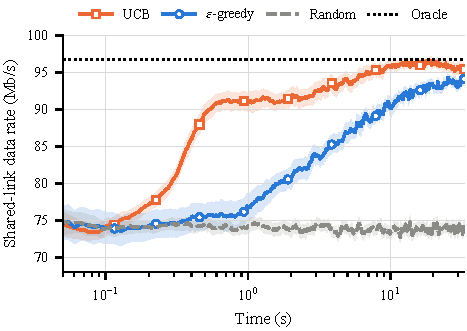
\includegraphics[width=\columnwidth]{fig_throughput.pdf}
\caption{Shared-link data rate of the urgency-agnostic schemes (30 runs, 50-TXOP moving average, 95\% confidence bands).}
\label{fig:rate}
\end{figure}

\begin{figure*}[t]
\centering
\subfigure[]{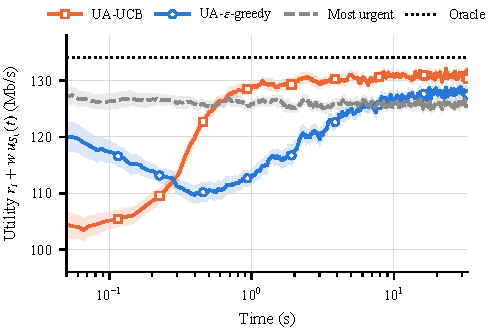
\includegraphics[width=0.48\textwidth]{fig_utility.pdf}\label{fig:utility}}
\hfill
\subfigure[]{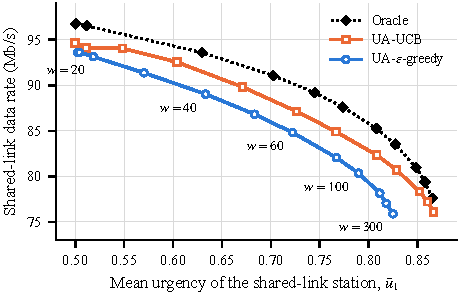
\includegraphics[width=0.48\textwidth]{fig_tradeoff.pdf}\label{fig:tradeoff}}
\caption{Urgency-aware schemes (30 runs). (a) Utility for $w=60$~Mb/s (50-TXOP moving average, 95\% confidence bands). (b) Steady-state rate versus $\bar{u}_1$. The markers on each curve correspond to $w=0$, 10, 20, 30, 40, 50, 60, 80, 100, 150, 200 and 300~Mb/s from left to right.}
\label{fig:aware}
\end{figure*}

\begin{table}[t]
\caption{Urgency-Agnostic Schemes (95\% Confidence Half-Width of $\bar{r}$ at Most 0.5~Mb/s)}
\label{tab:agnostic}
\centering
\footnotesize
\setlength{\tabcolsep}{4pt}
\begin{tabular}{@{}lcccccc@{}}
\toprule
Scheme & $\bar{r}$ (Mb/s) & $\bar{r}/\bar{r}^\star$ & $\bar{r}_{\mathrm{run}}$ (Mb/s) & $t_{50}$ (s) & $t_{90}$ (s) & $\pi^\star$\\
\midrule
Random & 73.85 & 76.3\% & 73.85 & n/a & n/a & 15.4\%\\
$\epsilon$-greedy & 93.66 & 96.8\% & 90.69 & 2.92 & 11.42 & 86.5\%\\
UCB & 95.53 & 98.8\% & 95.11 & 0.44 & 4.69 & 93.0\%\\
Oracle & 96.73 & 100\% & 96.73 & n/a & n/a & 100\%\\
\bottomrule
\end{tabular}
\end{table}

\begin{table}[t]
\caption{Sensitivity of the Urgency-Agnostic Schemes (95\% Confidence Half-Width of $\bar{r}$ at Most 1.5~Mb/s)}
\label{tab:sensitivity}
\centering
\footnotesize
\setlength{\tabcolsep}{4pt}
\begin{tabular}{@{}lccc@{\hspace{12pt}}lccc@{}}
\toprule
$\epsilon$ & $\bar{r}$ & $\bar{r}_{\mathrm{run}}$ & $\pi^\star$ & $c$ & $\bar{r}$ & $\bar{r}_{\mathrm{run}}$ & $\pi^\star$\\
\midrule
0 & 75.02 & 74.94 & 20.9\% & 0 & 90.99 & 90.84 & 68.1\%\\
0.02 & 90.88 & 86.18 & 70.0\% & 6 & 91.07 & 90.91 & 68.5\%\\
0.05 & 93.74 & 89.67 & 86.2\% & 12 & 92.69 & 91.77 & 77.0\%\\
0.1 & 93.66 & 90.69 & 86.5\% & 18 & 95.53 & 95.11 & 93.0\%\\
0.2 & 91.52 & 90.00 & 74.7\% & 24 & 95.23 & 92.18 & 92.1\%\\
0.3 & 89.29 & 88.39 & 64.6\% & 36 & 95.11 & 93.02 & 92.4\%\\
 & & & & 48 & 94.57 & 91.46 & 89.7\%\\
 & & & & 96 & 90.66 & 86.86 & 71.9\%\\
\bottomrule
\end{tabular}
\end{table}

\subsection{Urgency-Aware Schemes}
The UA schemes are compared with the most-urgent-first rule, which selects the most urgent candidate station without learning, and with the utility oracle \eqref{eq:oracleu}. For $w=60$~Mb/s (Fig.~\ref{fig:utility} and Table~\ref{tab:aware}), UA-UCB attains $\bar{U}=130.90$~Mb/s (97.7\% of $\bar{U}^w$) and UA-$\epsilon$-greedy 128.14~Mb/s (95.6\%). The most-urgent-first rule gives 125.84~Mb/s with $\bar{u}_1=0.87$ but only 73.55~Mb/s of rate. UA-UCB passes this rule after 0.57~s and UA-$\epsilon$-greedy after 5.89~s. The initial drop of UA-$\epsilon$-greedy occurs because tried arms, with $Q\approx r/2$ from \eqref{eq:ewma}, outrank untried arms regardless of urgency.

Fig.~\ref{fig:tradeoff} shows the rate against $\bar{u}_1$ for $w$ from 0 to 300~Mb/s. For every $w\geq10$~Mb/s, UA-UCB gives both a higher rate and a higher $\bar{u}_1$ than UA-$\epsilon$-greedy and stays closer to the oracle curve. In agreement with \eqref{eq:flip}, $w\leq10$~Mb/s, which is below the 17.8~Mb/s gap, has almost no effect. At $w=300$~Mb/s, UA-UCB reaches $\bar{u}_1=0.866$, close to the limit of 0.87 from \eqref{eq:ulimit}, while UA-$\epsilon$-greedy stops at 0.825 because of its random choices.

\begin{table}[t]
\caption{Urgency-Aware Schemes, $w=60$~Mb/s (95\% Confidence Half-Width of $\bar{U}$ and $\bar{r}$ at Most 0.21~Mb/s)}
\label{tab:aware}
\centering
\footnotesize
\setlength{\tabcolsep}{3pt}
\begin{tabular}{@{}lccccccc@{}}
\toprule
Scheme & $\bar{U}$ (Mb/s) & $\bar{U}/\bar{U}^w$ & $\bar{r}$ (Mb/s) & $\bar{u}_1$ & $t_{50}$ (s) & $t_{90}$ (s) & $\pi^w$\\
\midrule
Most urgent & 125.84 & 93.9\% & 73.55 & 0.87 & n/a & n/a & 46.4\%\\
UA-$\epsilon$-greedy & 128.14 & 95.6\% & 84.82 & 0.72 & 2.25 & 8.06 & 63.1\%\\
UA-UCB & 130.90 & 97.7\% & 84.92 & 0.77 & 0.43 & 1.03 & 69.3\%\\
Oracle & 134.03 & 100\% & 87.61 & 0.77 & n/a & n/a & 100\%\\
\bottomrule
\end{tabular}
\end{table}

\section{Conclusion}\label{sec5}
In this letter, we modeled two-AP C-SR in IEEE 802.11bn as a contextual selection problem and solved it with an H-MAB that learns from the observed data rate. UCB outperformed $\epsilon$-greedy in learning speed and steady-state rate and reached 98.8\% of the oracle rate. Adding a weighted urgency term to the selection index gave UA agents whose trade-off is set by a single weight, and UA-UCB reached 97.7\% of the oracle utility. Future work will include the sharing-link loss in the reward, larger C-SR groups and queue-based urgency.

\bibliographystyle{IEEEtran}
\bibliography{BBN_CL}
\end{document}
